\section{Plan}

We will retain day type, room type, their interaction, and city terms to answer our research question. For other predictors, we will use coefficient t-tests and partial F-tests for groups of terms. Correlations between distance measures (r = 0.56) and ratings (r = 0.71) motivate comparing models retaining one or both measures. Literature and context will guide selection; we will compare adjusted R\(^{2}\) on the same response scale and track the main interaction estimate.

All observed prices are positive, but 195 fitted prices are negative. Given the right-skewed response and unequal residual spread, we will consider Box--Cox transformations, likely log price, comparing residual patterns, spread, and Q--Q plots. With log price, we will compare weekend-to-weekday price ratios across room types. Predictor-specific curvature will motivate testing nonlinear terms. We will recheck all residual plots and both additional conditions after every model change.

Figure~\ref{fig:plan} gives responsibilities and milestones through December 2.

\begin{figure}[!htbp]
\centering
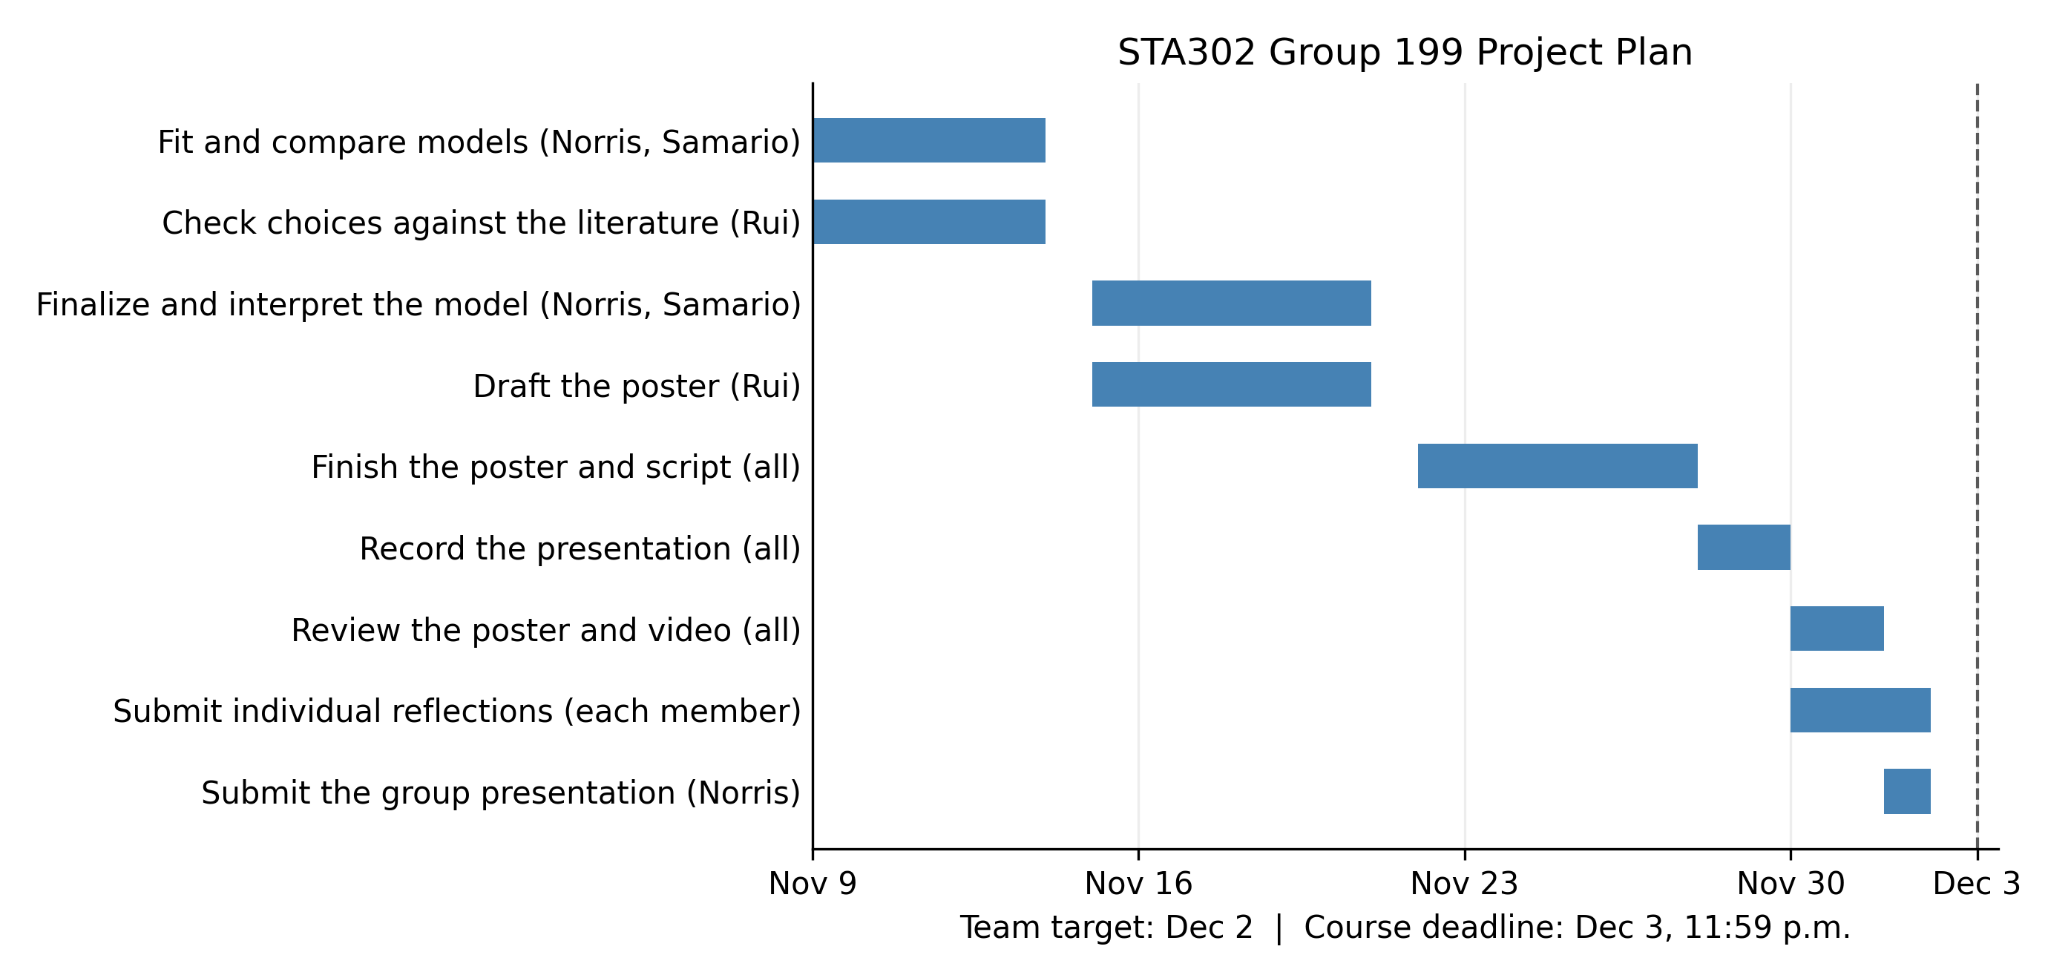
\includegraphics[width=\linewidth]{figures/04_team_schedule.png}
\caption{Team schedule and responsibilities.}
\label{fig:plan}
\end{figure}
